\documentclass{book}
\usepackage{background}
\usepackage{tikz}
\usepackage{fancyhdr}
\usepackage{tabularx}
\usepackage{graphicx}
\usepackage{geometry}
\usepackage{hyperref}
\usepackage{fontspec}
\usepackage{xcolor}
\usepackage{minted}
\usepackage{amsmath}
% Define colors
\definecolor{linkcolor}{RGB}{0,0,255}  % Blue color
\definecolor{citecolor}{RGB}{0,128,0}  % Green color
\definecolor{urlcolor}{RGB}{255,0,0}   % Red color

% Setup hyperlink colors
\hypersetup{
	colorlinks=true,
	linkcolor=linkcolor,
	citecolor=citecolor,
	urlcolor=urlcolor,
	linktoc=all
}

% setup geometry
\geometry{
	a4paper,
	left=2cm,
	right=2cm,
	top=2.5cm,
	bottom=2.5cm
}

% Set up background image
\backgroundsetup{
	scale=1,
	color=black,
	opacity=1,
	angle=0,
	position=current page.center,
	vshift=0cm,
	hshift=0cm,
	contents={
			\includegraphics[width=\paperwidth,height=\paperheight]{../jpgs/texture-min.jpg}
		}
}

% Custom headers and footers
\pagestyle{fancy}

% Necessary Details 🤠
\title{Computer Scientist in A Nutshell}
\author{Miskatul Anwar}

% Font configuration
\setmainfont{IosevkaTermSlab Nerd Font}

% Starting the document
\begin{document}
\maketitle
\newpage
\chapter{Maths}

Maths will be the foundation what you'll need the most in this journey!
The most important topics are \dots
\section{Permutations \& Combinations}
\textbf{Problems Related to Counting}
\begin{enumerate}
	\item Consider the word "Permutation". In how many ways can you arrange the letters,\\
	      \begin{itemize}
		      \item \textbf{No, rule specified,}\\
		            \[
			            Answer: \space n_t=2
		            \]
		            \[
			            \frac{11!}{2!}
		            \]
		      \item \textbf{If, The vowels stay together,\\}
		            \[
			            n_{total} = 7
		            \]
		            \[
			            n_t=2\\
		            \]
		            \[
			            The \space Answer:\space \frac{7!}{2!}\cdot 5!
		            \]
		      \item \textbf{If, The vowels don't stay together,\\}
		            \[
			            \frac{11!}{2!}-\frac{7!}{2!}\cdot 5!
		            \]
		      \item \textbf{If the vowels stay at their place,}\\
		            \[
			            \frac{6!}{2!}
		            \]
		      \item \textbf{If, The order (vowels) is same,}\\
		            "euaio" if the order of the vowels. Let's consider them as a single word.
		            \[
			            \frac{11!}{2!5!}
		            \]
		      \item \textbf{If the relative order is the same,}\\
		            \[
			            \frac{6!}{2!}\cdot 5!
		            \]
	      \end{itemize}
	\item How many numbers greater than 800 and less than 4000 can be made with the digits 0,1,2,4,5,7,8,9 ? (no number occuring more than once in the same number)\\
	      \textit{ Sol. }
	      firstly, let's consider the 801 - 999 range...(all the three digit numbers available in the limit)\\
	      The first number will definitely be 8 or 9, so the possible ways to put the first number is 2. The other numbers will be put as follows.
	      \[
		      2 \cdot 7 \cdot 6
	      \]
	      secondly, consider the 1000 - 3999 range...(all the four digit numbers available in the limit)\\
	      The first number can only be 1 or 2 as three  is not given. So, the rest will be declining in the previously shown manner.
	      \[
		      2 \cdot 7\cdot 6\cdot 5
	      \]
	      Now, calculation of the possible ways is as follows:
	      \[
		      2 \cdot 7 \cdot 6 + 2 \cdot 7\cdot 6\cdot 5 = 504
	      \]
	\item Your Home to DU there's 3 ways avalable to go. DU to BUET there's only 2 available ways. How many ways are there to visit BUET from your home?\\
	      (Yeah, ugh\dots you have'nt got a chance to read in BUET)\\
	      \textit{ Sol=> } There are 6 different ways to visit BUET from your home.
	\item there are five people in a vehicle. But there is only three sits available. In how many ways we can pick 3 people to have their sits?\\
	      \textit{ Sol.=> } The answer is:
	      \[
		      5 \cdot 4 \cdot 3 = 60
	      \]
	      If we apply the formulae,
	      pick 3 people from 5 and arrange them.
	      \[
		      ^5P_3 = 60
	      \]
	\item How many even numbers of three digits can be formed from the digits 0,1,2,3,4,5,6 ?\\
	      \textit{ Sol.1} If the last digit is 0, 2, 4 or 6 , then it can be an even number. Also, we need to keep in mind that
	      the first number can't be zero.
	      \[
		      6 \cdot 5 \cdot 1 + 5 \cdot 5 \cdot 3 = 105
	      \]
	\item  The following problems have to do with cardinalities of sets
	      of phone numbers of certain kinds.
	      \begin{itemize}
		      \item How many 7-digit phone numbers are possible, assuming
		            that the first digit can’t be a 0 or a 1?\\
		            \textit{ Sol. }\\
		            To determine the number of possible 7-digit phone numbers where the first digit cannot be 0 or 1, we can break the problem into parts:\\
		            \begin{itemize}
			            \item First Digit: The first digit has 8 possible choices (2 through 9).
			            \item Remaining Digits: Each of the remaining 6 digits can be any digit from 0 to 9, giving each position 10 possible choices.
		            \end{itemize}

		            Therefore, the total number of 7-digit phone numbers can be calculated as follows:\\
		            \[
			            8 \cdot 10^6
		            \]

		            Here's the step-by-step calculation:\\
		            There are 8 choices for the first digit.
		            There are 10 choices for each of the remaining 6 digits.
		            So, multiplying these together:
		            \[
			            8\cdot10^6=8,000,000
		            \]

		            Thus, there are 8,000,000 possible 7-digit phone numbers under the given constraints.
		      \item  Solve the above problem again, except now assume also that
		            the phone number is not allowed to start with 911 (since
		            this is reserved for emergency use, and it would not be
		            desirable for the system to wait to see whether more digits
		            were going to be dialed after someone has dialed 911).
		            \textit{ Sol. }\\
		            To solve this problem under the new constraints, we need to calculate the total number of valid 7-digit phone numbers that do not start with 911.\\
		            \textbf{Steps:}
		            \begin{enumerate}
			            \item Total number of 7-digit phone numbers without additional constraints:
			                  As previously calculated, the total number of possible 7-digit phone numbers where the first digit can't be 0 or 1 is:
			                  \[
				                  8×10^6
				                  =8,000,000
			                  \]
			            \item Calculate the number of invalid phone numbers that start with 911:
			                  \begin{itemize}
				                  \item If the phone number starts with 911, the first three digits are fixed as 911.
				                  \item The remaining 4 digits can each be any digit from 0 to 9, so there are
				                        10 choices for each of the remaining 4 digits.
			                  \end{itemize}
			                  Therefore, the number of phone numbers that start with 911 is:
			                  \[
				                  10
				                  ×
				                  10
				                  ×
				                  10
				                  ×
				                  10
				                  =
				                  1
				                  0
				                  ^4
				                  =
				                  10
				                  ,
				                  000
			                  \]

		            \end{enumerate}
		      \item Subtract the number of invalid phone numbers from the total:\\

		            Total valid phone numbers = Total possible phone numbers - Invalid phone numbers.\\
		            \[
			            8,000,000−10,000=7,990,000
		            \]
	      \end{itemize}
	      Thus, the total number of valid 7-digit phone numbers, ensuring the first digit can't be 0 or 1 and the number does not start with 911, is 7,990,000.
	\item How many different functions f : A → B are possible in total
	      with |A| = m and |B| = n? (m and n are, of course, positive
	      integers.)\\
	      \textit{ Sol.2}\\

	      To determine how many different functions
	      f:A→B are possible with
	      ∣A∣=m and ∣B∣=n, we can consider the following:
	      \begin{itemize}
		      \item
		            Definition of a Function: A function
		            \[
			            f:A\rightarrow B
		            \] maps every element in set
		            A to an element in set
		            B.
		      \item
		            Total Number of Functions:

		            For each element in set
		            A, there are
		            n possible choices in set
		            B.
		            Since there are
		            m elements in set
		            A, each of the
		            m elements can independently be mapped to any of the
		            n elements in
		            B.

	      \end{itemize}

	      To find the total number of such functions, we use the principle of counting:
	      \[
		      n×n×n×⋯×n(m times)
	      \]

	      This can be written as:
	      \[
		      n^m
	      \]
	      Conclusion
	      Thus, the total number of different functions
	      f:A→B with
	      ∣A∣=m and
	      ∣B∣=n is
	      \[
		      n^m
	      \]
	\item
	      \begin{itemize}
		      \item  Consider the grid shown below. Starting at a point, you can
		            go one step up or one step to the right at each move (as long
		            as any such move keeps you within the grid). This procedure
		            is continued until the point C is reached from point A.\\
		            (a) How many different paths are there from A to C?\\
		            (b) How many different paths from A to C pass through B?\\
		            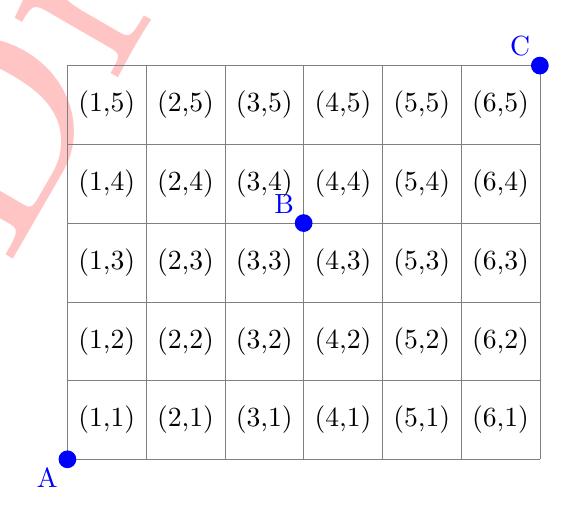
\begin{tikzpicture}
			            % Grid lines
			            \draw[step=1cm,gray,very thin] (0,0) grid (6,5);

			            % Points A, B, C
			            \filldraw[blue] (0,0) circle (3pt) node[anchor=north east] {A};
			            \filldraw[blue] (3,3) circle (3pt) node[anchor=south east] {B};
			            \filldraw[blue] (6,5) circle (3pt) node[anchor=south east] {C};

			            % Labels for grid points
			            \foreach \x in {1,...,6} {
					            \foreach \y in {1,...,5} {
							            \node at (\x-0.5,\y-0.5) {(\x,\y)};
						            }
				            }\end{tikzpicture}\\
		            (We say that two paths are different whenever they are not
		            identical.)\\

		            Let's analyze the problem of finding different paths in a 5x6 grid from point A to point C, and specifically how many of those paths pass through point B(2,3).
		            In a 5x6 grid:\\
		            Starting from point A(1,1) to point C(5,6), you need to make 4 steps up and 5 steps to the right.
		            The total number of paths from A to C can be calculated using the combination formula, since each path consists of 4 up movements (U) and 5 right movements (R):
		            \[
			            Total Paths = 9C4
		            \]
		            Calculating this:
		            \[
			            \frac{4×3×2×1}{9×8×7×6} =126
		            \]
		            So, there are 126 different paths from A to C in the grid.
		      \item
		            To find paths from A to C that pass through B(2,3):

		            From A to B(2,3), you need 1 step up and 2 steps to the right.
		            From B(2,3) to C(5,6), you need 3 steps up and 3 steps to the right.
		            So, the paths from A to C passing through B(2,3) involve:\\

		            1 step up from A to B,\\
		            2 steps to the right from A to B,\\
		            3 steps up from B to C, and\\
		            3 steps to the right from B to C.\\
		            This gives a total of:
		            \[
			            3C1 \cdot 5C2 = 30
		            \]
		            \begin{itemize}
			            \item  There are 126 different paths from A to C.
			            \item There are 30 different paths from A to C that pass through B(2,3).
		            \end{itemize}
	      \end{itemize}
	\item As a part of the population in Silverland seeks to break free,
	      higher ups of the mafia enterprise that controls Silverland has
	      decided to quickly form a regional subcommittee with their
	      operatives to teach them a lesson. The subcommittee is to
	      consist of 3 hockeystick experts (H), 2 tech-savvy social media
	      monitors (S), and 2 specializing in effective usage of machete
	      (M). When a pool of 8 H, 3 S, and 6 M among their regular
	      thugs in the territory are available, in how many different
	      ways the subcommittee can be formed if
	      \begin{itemize}
		      \item \textbf{(a) 2 of the H refuse to serve together:}

		            Total ways without restriction:
		            \[ \binom{8}{3} \times \binom{3}{2} \times \binom{6}{2} \]

		            Ways with 2 specific H serving together:
		            \[ \binom{6}{1} \times \binom{3}{2} \times \binom{6}{2} \]

		            Number of ways where the 2 H do not serve together:
		            \[
			            \binom{8}{3} \times \binom{3}{2} \times \binom{6}{2} - \left( \binom{6}{1} \times \binom{3}{2} \times \binom{6}{2} \right)
		            \]
		      \item \textbf{(b) 2 of the M refuse to serve together:}

		            Total ways without restriction:
		            \[ \binom{8}{3} \times \binom{3}{2} \times \binom{6}{2} \]

		            Ways with 2 specific M serving together:
		            \[ \binom{8}{3} \times \binom{3}{2} \times \binom{4}{2} \]

		            Number of ways where the 2 M do not serve together:
		            \[
			            \binom{8}{3} \times \binom{3}{2} \times \binom{6}{2} - \left( \binom{8}{3} \times \binom{3}{2} \times \binom{4}{2} \right)
		            \]
		      \item \textbf{(c) 1 S and 1 M refuse to serve together:}

		            Total ways without restriction:
		            \[ \binom{8}{3} \times \binom{3}{2} \times \binom{6}{2} \]

		            Ways with 1 specific S and 1 specific M serving together:
		            \[ \binom{8}{3} \times \binom{2}{1} \times \binom{5}{1} \times \binom{5}{2} \]

		            Number of ways where 1 S and 1 M do not serve together:
		            \[
			            \binom{8}{3} \times \binom{3}{2} \times \binom{6}{2} - \left( \binom{8}{3} \times \binom{2}{1} \times \binom{5}{1} \times \binom{5}{2} \right)
		            \]
	      \end{itemize}
\end{enumerate}
\end{document}
